\documentclass[11pt]{beamer}
\usepackage[utf8]{inputenc}
\usepackage[spanish]{babel}
%\usepackage{amsmath}
%\usepackage{amsfonts}
%\usepackage{amssymb}
%\usepackage{graphicx}
\usepackage{subfigure} % subfiguras
\usepackage{ragged2e}
%\usepackage{hyperref}
\usepackage{float}
\usepackage{url}
\usepackage{listings}
%\usepackage{xcolor}
\usepackage{algorithm,algorithmic}

\usepackage{mathtools}
\DeclarePairedDelimiter\ceil{\lceil}{\rceil}
\DeclarePairedDelimiter\floor{\lfloor}{\rfloor}

\usepackage{color}
\definecolor{lightgray}{rgb}{.9,.9,.9}
\definecolor{darkgray}{rgb}{.4,.4,.4}
\definecolor{purple}{rgb}{0.65, 0.12, 0.82}

\lstdefinelanguage{JavaScript}{
  keywords={typeof, new, true, false, catch, function, return, null, catch, switch, var, if, in, while, do, else, case, break},
  keywordstyle=\color{blue}\bfseries,
  ndkeywords={class, export, boolean, throw, implements, import, this},
  ndkeywordstyle=\color{darkgray}\bfseries,
  identifierstyle=\color{black},
  sensitive=false,
  comment=[l]{//},
  morecomment=[s]{/*}{*/},
  commentstyle=\color{purple}\ttfamily,
  stringstyle=\color{red}\ttfamily,
  morestring=[b]',
  morestring=[b]"
}

\lstset{
   language=JavaScript,
   backgroundcolor=\color{lightgray},
   extendedchars=true,
   basicstyle=\tiny\ttfamily,
   %basicstyle=\footnotesize\ttfamily,
   showstringspaces=false,
   showspaces=false,
   numbers=left,
   numberstyle=\footnotesize,
   numbersep=4pt,
   tabsize=1,
   breaklines=true,
   showtabs=false,
   captionpos=b
}

\usetheme{Madrid}

%\usepackage{natbib}
\usepackage{bibentry}
\usepackage{graphicx} % Allows including images
\usepackage{booktabs} % Allows the use of \toprule, 

\setbeamertemplate{bibliography item}{\insertbiblabel}

\newcommand{\celda}[1]{
	\begin{minipage}{2.5cm}
		\vspace{5mm}
		#1
		\vspace{5mm}
	\end{minipage}
}

\author[Abarca, Apari, Suca, Vargas] % (optional)
{J.~P.~Abarca\inst{1} \and C.~T.~Apari\inst{1} \and C.~A.~Suca\inst{1} \and A.~Vargas\inst{1}  }
\title[Practica2]{Práctica 2}
\date{ 03 de Julio del 2021} 
%\date{\currenttime}
\subtitle{Estructura de Datos}
\logo{
\includegraphics[scale=0.16]{unsa.png}}
\institute[UNSA]{
	\inst{1}
		Universidad Nacionan del San Agustin. Facultad de Producción y Servicios. \\Escuela Profesional de Ciencias de la Computación\\
		Maestría en Ciencias de la Computación \\ Docente: Mg. Vicente Machaca \\
		\vspace{2mm}
}

\AtBeginSection[]
{
	\begin{frame}<beamer>{Contenido}
		\tableofcontents[currentsection,currentsubsection]
	\end{frame}
}

\begin{document}
	
	\begin{frame}
		\maketitle
	\end{frame}

	\begin{frame}{Contenido}
		\tableofcontents
	\end{frame}
	
    %%%%% ARBOL AVL
    \section{Arbol AVL}
	\subsection{Rotación}
	\begin{frame}{Reglas de rotación}
			\justifying
			\begin{figure}[H]
				\centering
				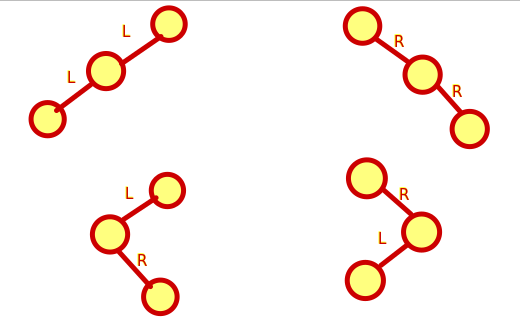
\includegraphics[scale=0.40]{img/rotacionavl.png}
				\caption{4 tipos de rotaciones \cite{DS2008}}
				\label{fig:rotacionavl}
			\end{figure}
		\end{frame}
	\begin{frame}{Rotación a la izquierda}
			\justifying
			
			\lstinputlisting[language=JavaScript, firstline=33, lastline=40, caption=Rotación a la izquierda]{code/tree-creation.js}
			
		\end{frame}
	\begin{frame}{Rotación a la derecha}
		\justifying
		
		\lstinputlisting[language=JavaScript, firstline=93, lastline=100, caption=Rotación a la derecha]{code/tree-creation.js}
		
	\end{frame}
	\subsection{Inserción}
		\begin{frame}{Insertar un elemento}
		\justifying
		
		\lstinputlisting[language=JavaScript, firstline=228, lastline=252, caption=Inserción de un elemento]{code/tree-creation.js}
		
	\end{frame}
		
	\subsection{Eliminación}
		\begin{frame}{Eliminación de un elemento}
			\justifying
			\begin{enumerate}
                \item Buscar en el subárbol izquierdo el nodo mayor, eliminar el nodo hallado y reemplazar el valor del nodo con el nodo a eliminar.
                \item Buscar en el subárbol derecho el nodo menor, eliminar el nodo hallado y reemplazar el valor del nodo con el nodo a eliminar.
            \end{enumerate}
			\begin{figure}[H]
				\centering
				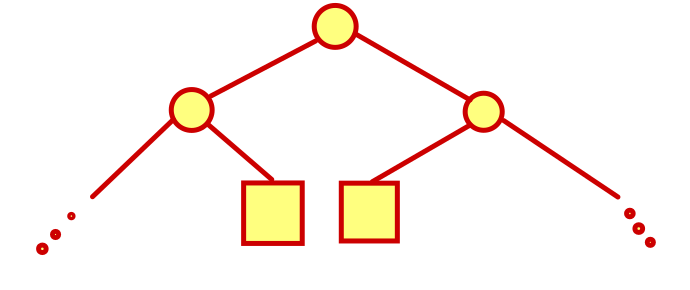
\includegraphics[scale=0.40]{img/eliminar.png}
				\caption{Eliminación de un nodo}
				\label{fig:eliminar}
			\end{figure}
			
		\end{frame}
	
	\subsection{Búsqueda}
		\begin{frame}{Búsqueda de un elemento}
			\justifying
			\lstinputlisting[language=JavaScript, firstline=498, lastline=518, caption=Búsqueda de un elemento]{code/tree-creation.js}
		\end{frame}
		
	%%%% ARBOL B
	\section{Arbol B}
	    \subsection{Búsqueda} %%% considerar el maximo y el minimo
		\begin{frame}{Búsqueda}
			\justifying
			\lstinputlisting[language=JavaScript, firstline=26, lastline=29, caption=Buscar en árbol]{code/btree.js}
			
			\lstinputlisting[language=JavaScript, firstline=18, lastline=32, caption=Desplazamiento]{code/btree-node.js}
			
		\end{frame}
		
		\begin{frame}{Búsqueda}
			\justifying
			\lstinputlisting[language=JavaScript, firstline=26, lastline=29, caption=Buscar en árbol]{code/btree.js}
			
			\lstinputlisting[language=JavaScript, firstline=18, lastline=32, caption=Desplazamiento]{code/btree-node.js}
			
		\end{frame}
		
		\begin{frame}{Búsqueda}
			\justifying
			\begin{figure}[H]
				\centering
				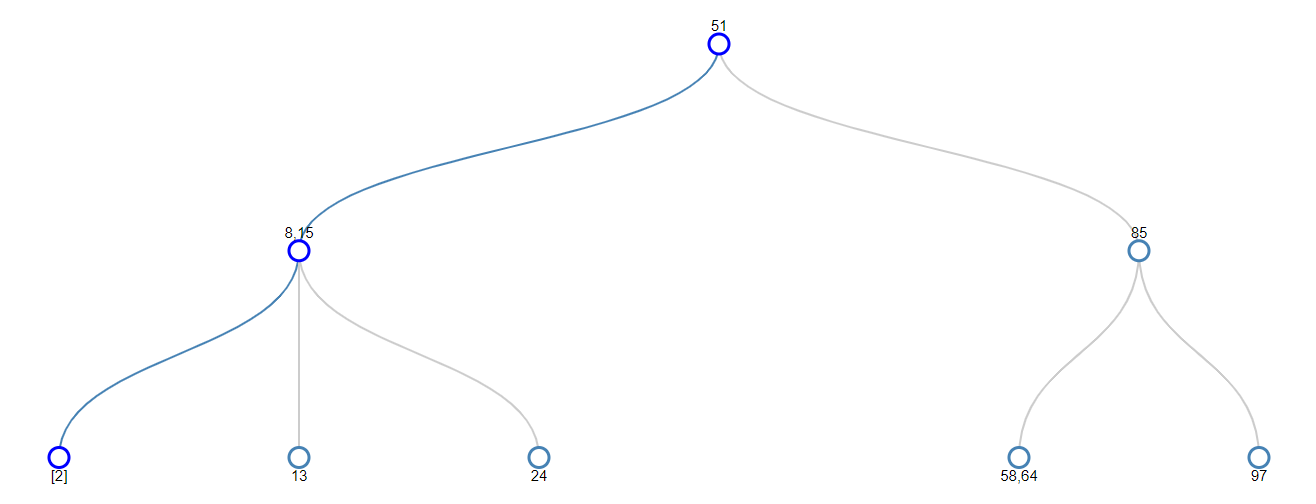
\includegraphics[scale=0.35]{img/btree_bus_1.png}
				\caption{Buscar en árbol}
				\label{fig:btree_bus_1}
			\end{figure}
		\end{frame}
		
		\begin{frame}{Máximo}
			\justifying
			\begin{figure}[H]
				\centering
				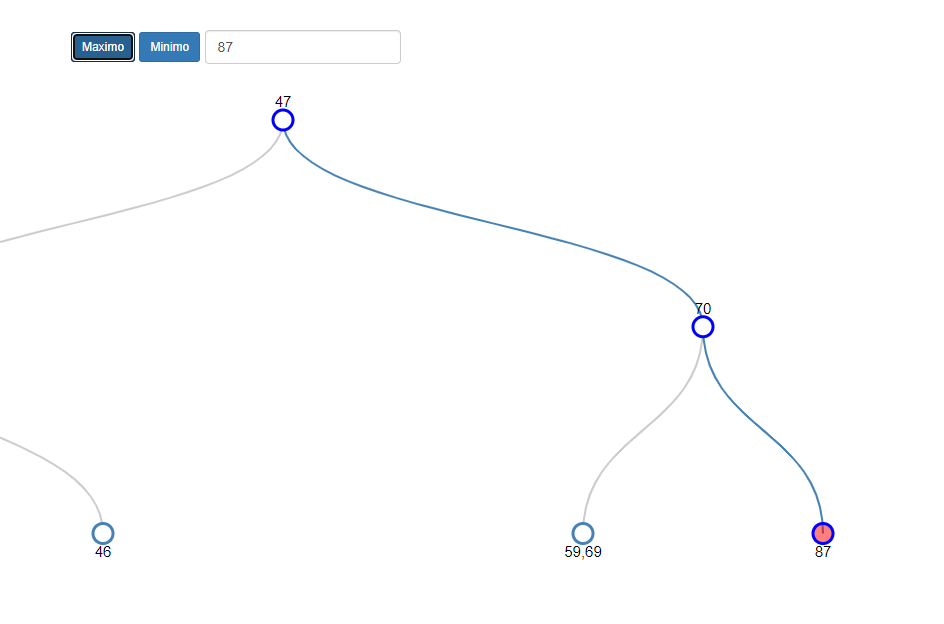
\includegraphics[scale=0.35]{img/btree_bus_2.png}
				\caption{Buscar Máximo}
				\label{fig:btree_bus_2}
			\end{figure}
		\end{frame}
		
		\begin{frame}{Mínimo}
			\justifying
			\begin{figure}[H]
				\centering
				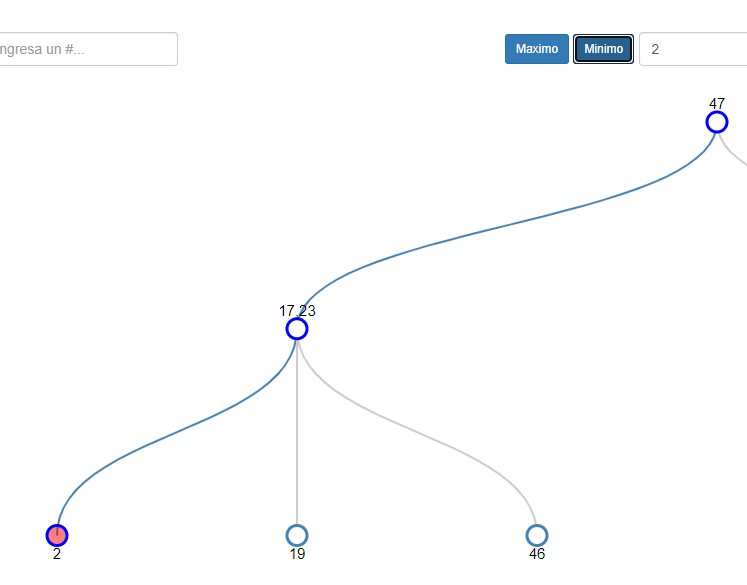
\includegraphics[scale=0.35]{img/btree_bus_3.png}
				\caption{Buscar Mínimo}
				\label{fig:btree_bus_3}
			\end{figure}
		\end{frame}
		
		\subsection{Inserción}
		\begin{frame}{Inserción}
			\justifying
			\lstinputlisting[language=JavaScript, firstline=32, lastline=55, caption=Inserción]{code/btree.js}
		\end{frame}
		
		\begin{frame}{Insertar en nodo (1)}
			\justifying
			\lstinputlisting[language=JavaScript, firstline=59, lastline=75, caption=Insertar en Nodo 1]{code/btree-node.js}
		\end{frame}
		\begin{frame}{Insertar en nodo (2)}
			\justifying
			\lstinputlisting[language=JavaScript, firstline=76, lastline=89, caption=Insertar en Nodo 2]{code/btree-node.js}
		\end{frame}
		
		\begin{frame}{Dividir(split)}
			\justifying
			\lstinputlisting[language=JavaScript, firstline=264, lastline=282, caption=Dividir en caso de overflow]{code/btree-node.js}
		\end{frame}
		
		\begin{frame}{Insertar nodo (1)}
			\justifying
			\begin{figure}[H]
				\centering
				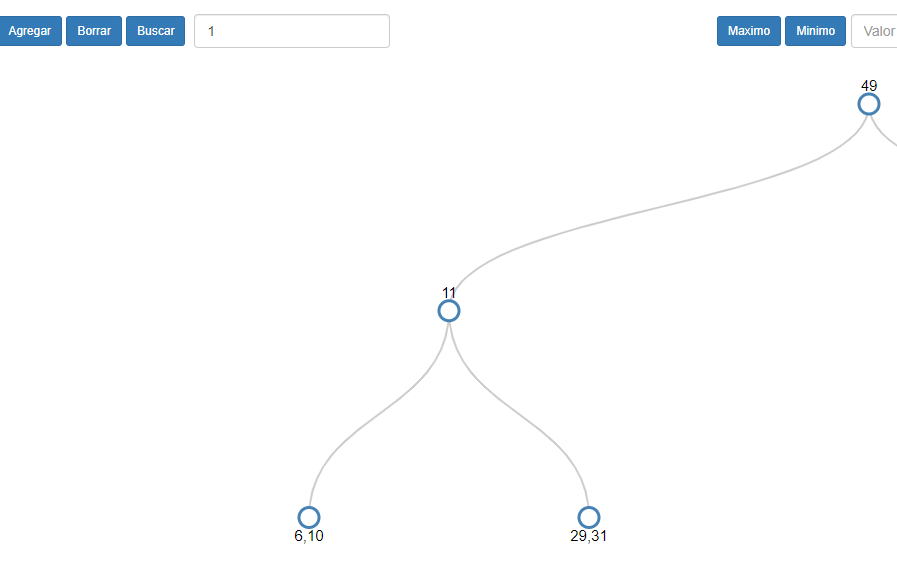
\includegraphics[scale=0.35]{img/btree_ins_1.png}
				\caption{Insertar nodo $key=1$ (1)}
				\label{fig:btree_ins_1}
			\end{figure}
		\end{frame}
		
		
		\begin{frame}{Insertar nodo (2)}
			\justifying
			\begin{figure}[H]
				\centering
				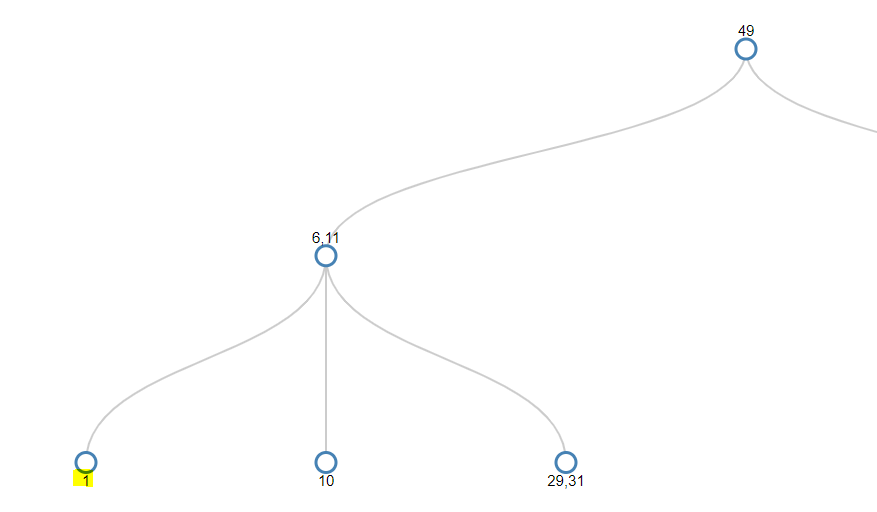
\includegraphics[scale=0.35]{img/btree_ins_2.png}
				\caption{insertar nodo $key=1$ (2)}
				\label{fig:btree_ins_2}
			\end{figure}
		\end{frame}
		
		
		\subsection{Eliminación}
		\begin{frame}{Reglas de eliminación}
			\justifying
            \begin{enumerate}
                \item Un nodo puede tener un número m máximo de hijos
                \item Un nodo puede tener un máximo de $m-1$ Claves (Keys)
                \item Un nodo debería tener un mínimo de $\ceil*{m/2}$ hijos
                \item Un nodo (excepto el nodo raíz) debería contener un mínimo de $\ceil*{m/2}-1$ Claves (Keys)
            \end{enumerate}
			
		\end{frame}
		
		%%% CASO 1
		\begin{frame}{Eliminar - Caso 1}
			\justifying
			
			\lstinputlisting[language=JavaScript, firstline=99, lastline=105, caption=Caso 1]{code/BTree-delete.js}
			
		\end{frame}
		
		\begin{frame}{Eliminar - Caso 1}
			\justifying
			\begin{figure}[H]
				\centering
				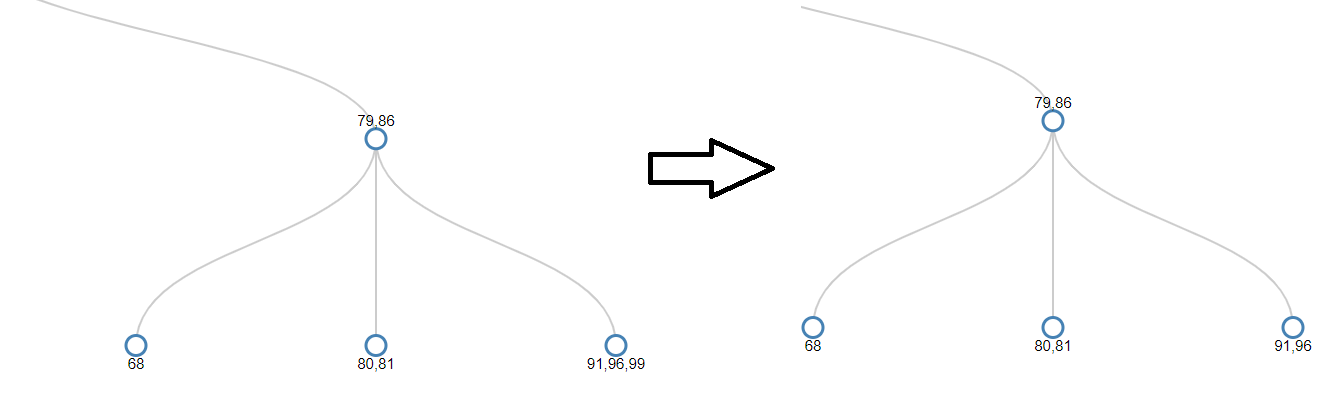
\includegraphics[scale=0.35]{img/btree_del_1.png}
				\caption{Caso 1 de Borrado de $Key=99$ en hoja sin problema \cite{CLRS2009}}
				\label{fig:btree_del_1}
			\end{figure}
		\end{frame}
		
		
		%%% CASO 2
		\begin{frame}{Eliminar - Caso 2}
			\justifying
			
			\lstinputlisting[language=JavaScript, firstline=106, lastline=124, caption=Caso 2]{code/BTree-delete.js}
			
		\end{frame}
		
		\begin{frame}{Eliminar - Caso 2}
			\justifying
			\begin{figure}[H]
				\centering
				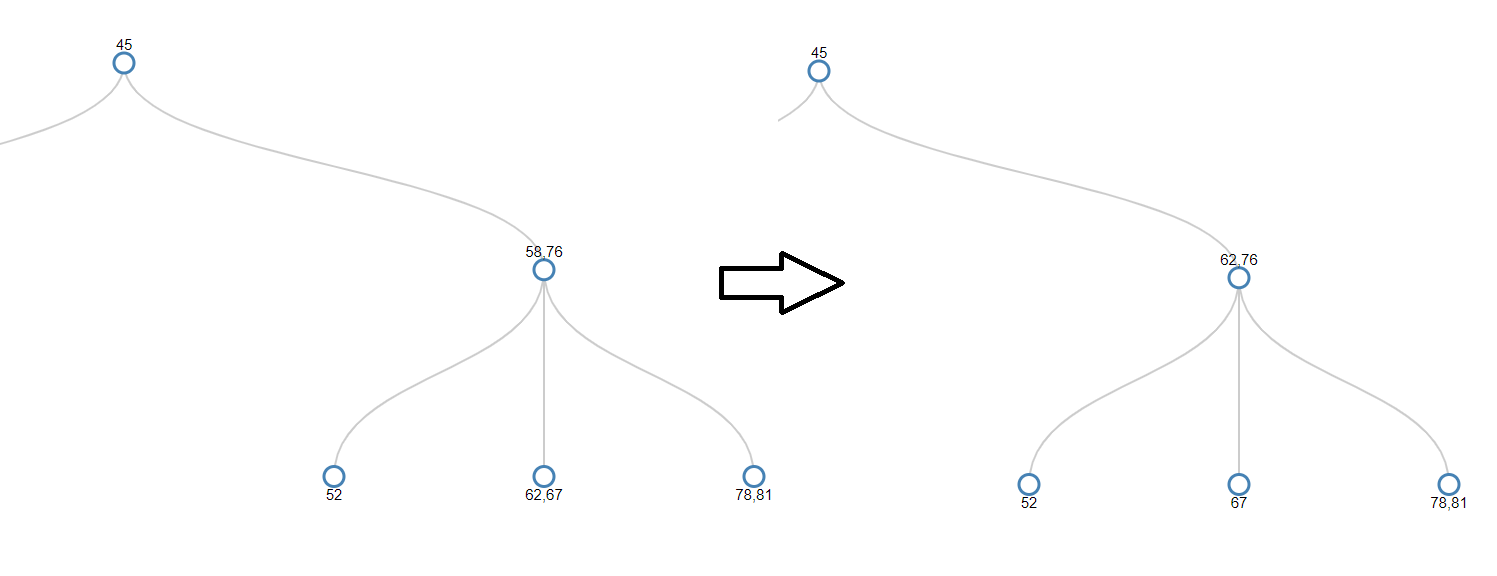
\includegraphics[scale=0.30]{img/btree_del_2.png}
				\caption{Caso 1 de Borrado $Key=58$ esta en el nodo \cite{CLRS2009}}
				\label{fig:btree_del_2}
			\end{figure}
		\end{frame}
		
		%%% CASO 3
		\begin{frame}{Eliminar - Caso 3}
			\justifying
			
			\lstinputlisting[language=JavaScript, firstline=125, lastline=138, caption=Caso 3]{code/BTree-delete.js}
			
		\end{frame}
		
		\begin{frame}{Eliminar - Caso 3}
			\justifying
			\begin{figure}[H]
				\centering
				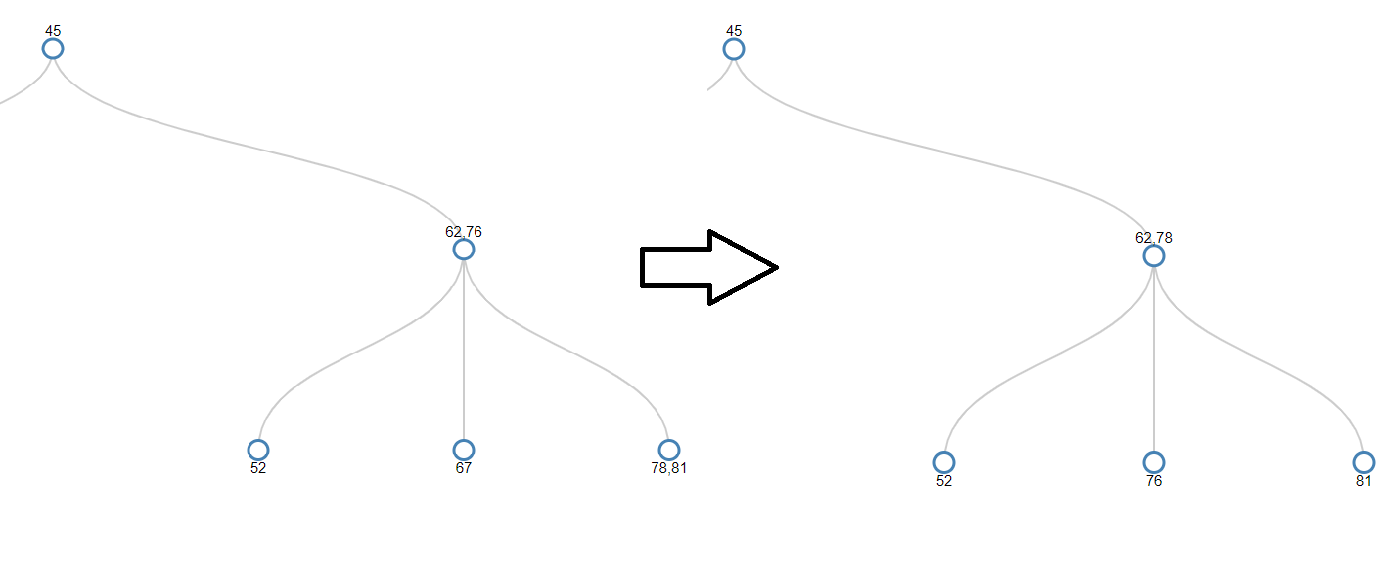
\includegraphics[scale=0.30]{img/btree_del_3.png}
				\caption{Caso 1 de Borrado Valor $Key=67$ no presente en el nodo \cite{CLRS2009}}
				\label{fig:btree_del_3}
			\end{figure}
		\end{frame}
		
		
		
		%%% ANIMACION BTREE
		\begin{frame}{Animación Btree}
			\justifying
			\begin{figure}[H]
				\centering
				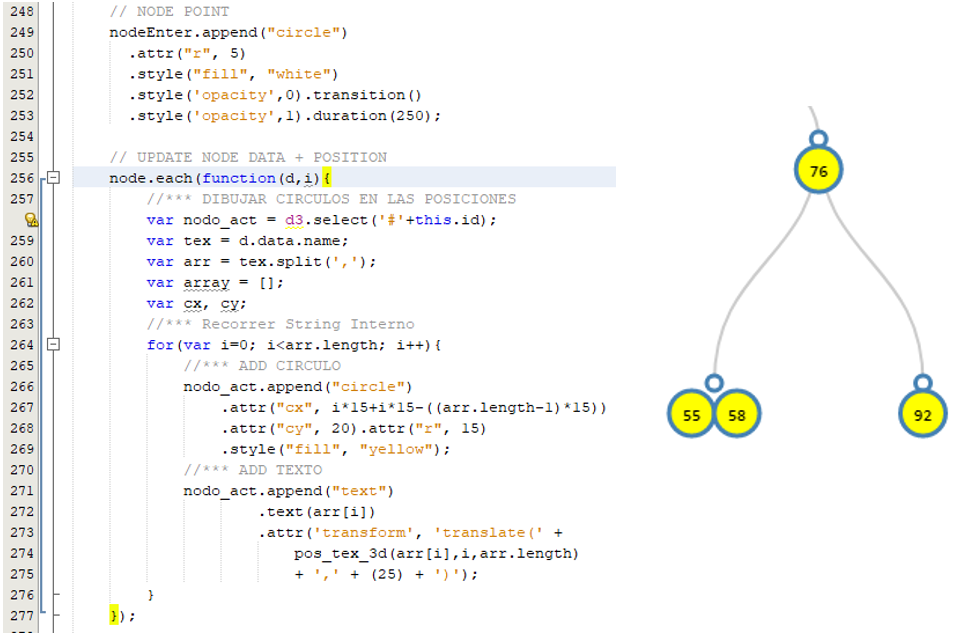
\includegraphics[scale=0.40]{img/btree_ani_1.PNG}
				\caption{Distribución de Claves (keys)}
				\label{fig:btree_ani_1}
			\end{figure}
		\end{frame}
		
		\begin{frame}{Animación Btree}
			\justifying
			\begin{figure}[H]
				\centering
				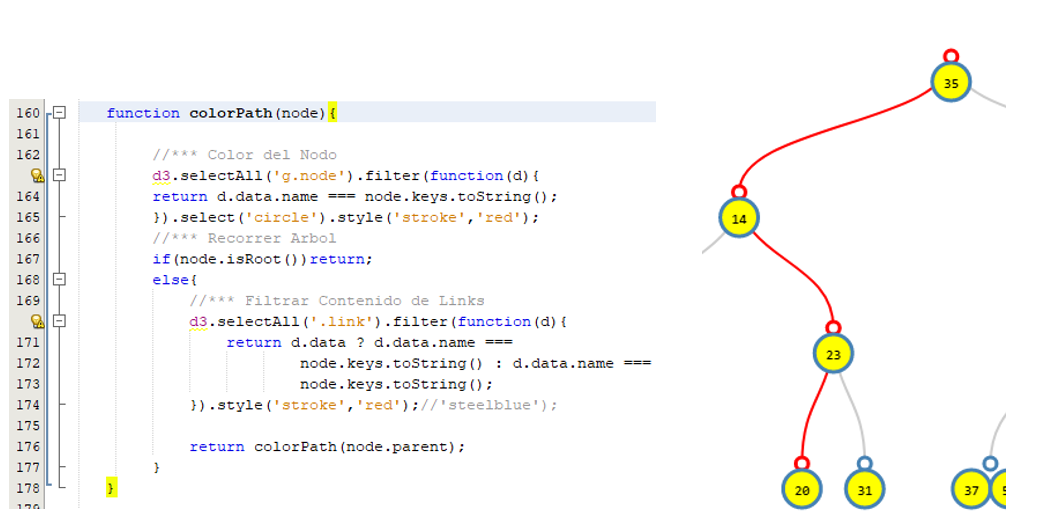
\includegraphics[scale=0.45]{img/btree_ani_2.PNG}
				\caption{Animación de Búsqueda}
				\label{fig:btree_ani_2}
			\end{figure}
		\end{frame}
		
		\begin{frame}{Animación Btree}
			\justifying
			\begin{figure}[H]
				\centering
				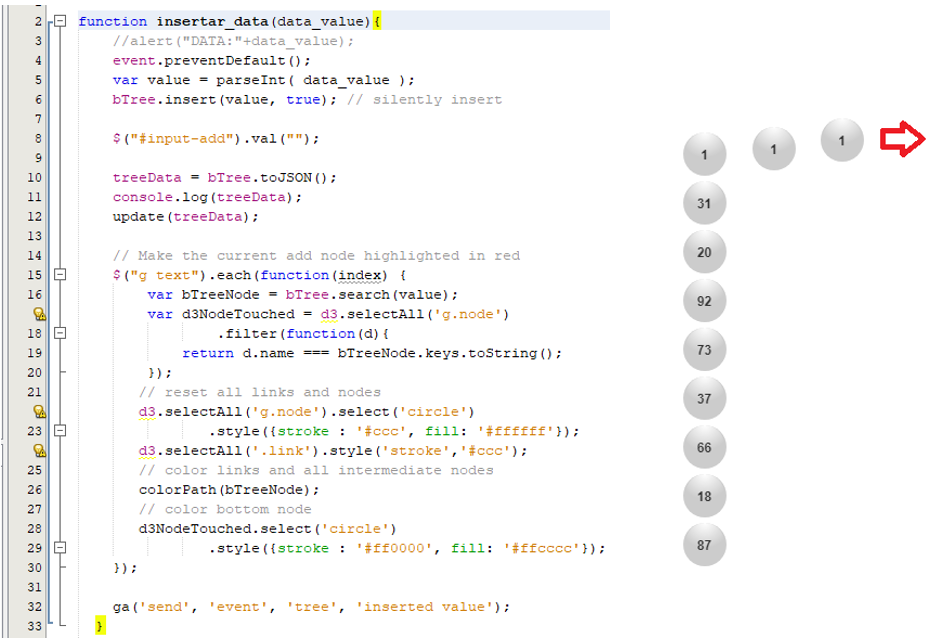
\includegraphics[scale=0.45]{img/btree_ani_3.PNG}
				\caption{Animación de Búsqueda}
				\label{fig:btree_ani_3}
			\end{figure}
		\end{frame}
		
		
		
		
		\begin{frame}{}
		    \centering
		    
		    {
		        \Large
		        GRACIAS
		    }
		    
		    \begin{figure}[H]
				\centering
				
\includegraphics[scale=0.5]{img/qr_repositorio.png}
				
				\label{fig:qr_repositorio}
			\end{figure}
			
			Repositorio: \url{https://github.com/jabarcamu/EDA_Practica2}
		    
		\end{frame}

%\appendix
\section{Referencias}
%\subsection<presentation>*{Referencias}

% All of the following is optional and typically not needed. 
%\appendix


\begin{frame}[t, allowframebreaks]
    \frametitle{References}
    \bibliographystyle{ieeetr}
    \bibliography{biblio}
\end{frame}



\end{document}